%*****************************************
\chapter{Methods}\label{ch:methods}
%*****************************************
For much of this thesis, single-compartment model neurons with Hodgkin-Huxley type membrane currents and an intracellular calcium buffer were used\autocite{HodgkinMeasurementcurrentvoltagerelations1952, Hodgkincomponentsmembraneconductance1952, Hodgkinquantitativedescriptionmembrane1952}. Similar models have been described previously\autocite{Liumodelneuronactivitydependent1998, PrinzAlternativehandtuningconductancebased2003, PrinzSimilarnetworkactivity2004, SoofiPhasemaintenancerhythmic2014}. The membrane currents are based on experiments on \textit{Homarus} neurons\autocite{TurrigianoSelectiveregulationcurrent1995}. 

Briefly, the currents consist of a \ac{INa}, a \ac{ICaT}, a \ac{ICaS}, a \ac{IA}, a \ac{IKCa}, a \ac{IKd}, a \ac{IH}, and a \ac{Ileak}.

\section{Model Parameters}
Model parameters were adapted from \autocite{PrinzAlternativehandtuningconductancebased2003, PrinzSimilarnetworkactivity2004}

\begin{figure}[h]
	\centering
	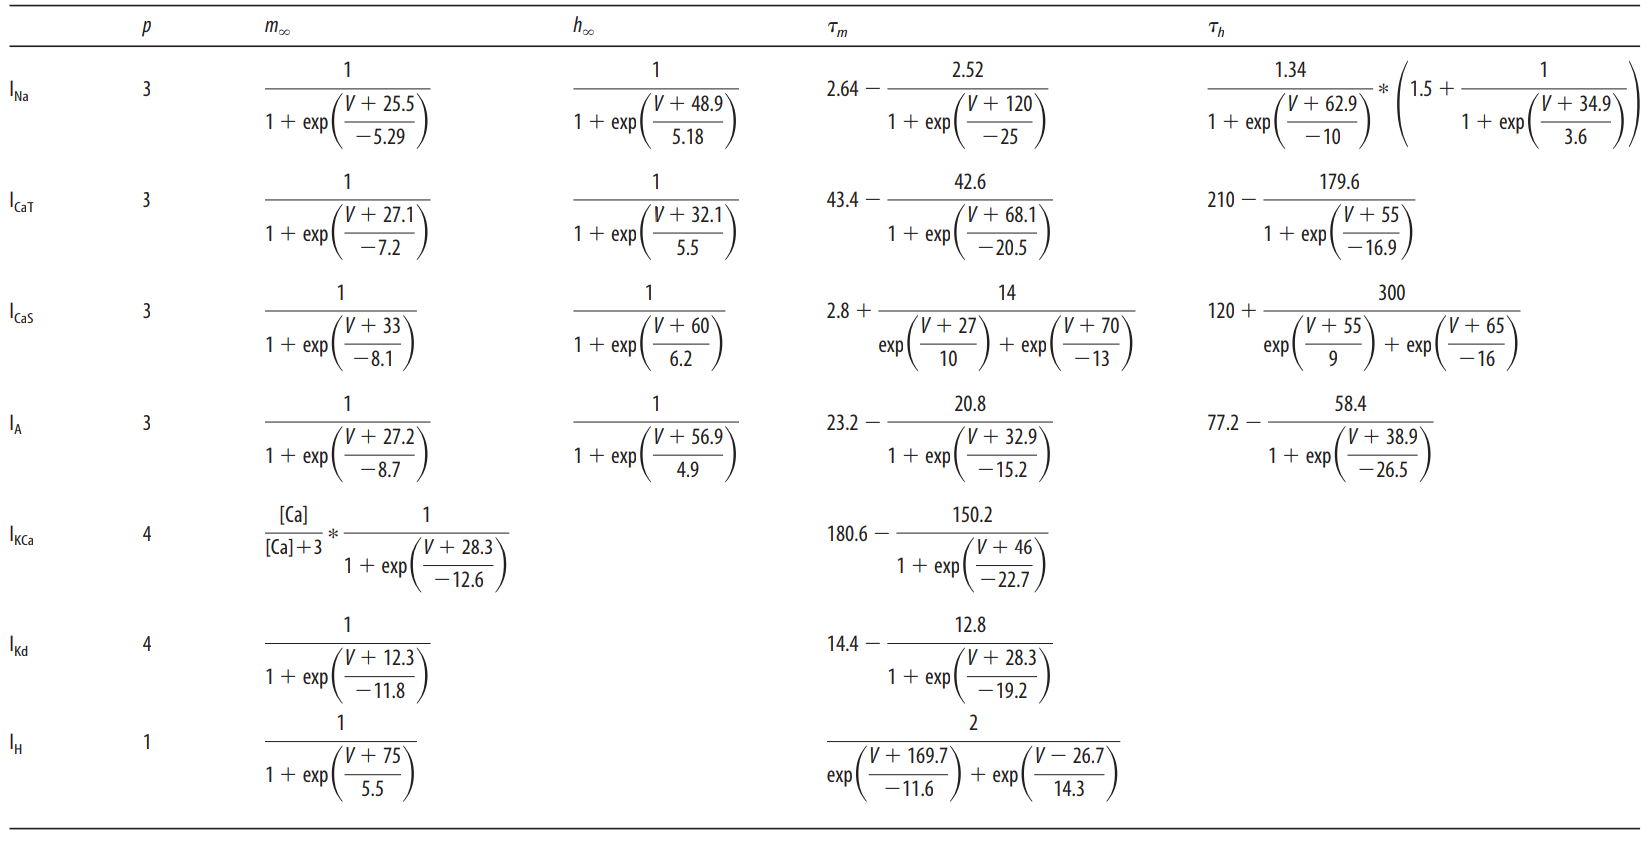
\includegraphics[width=1.0\linewidth]{gfx/VoltageDependence}
	\caption[Voltage dependence for model currents]{Voltage dependence of model currents. $V$ is the membrane potential in mV; $[Ca]$, the intracellular calcium concentration in mM. Absences in the table indicate non-inactivating currents (e.g. $h = 1 ~\forall~ V$).}
	\label{fig:voltagedependence}
\end{figure}

%\begin{table}[h]
%	\myfloatalign
%	\begin{tabularx}{\textwidth}{cccccc} \toprule
%		& p & $m_\infty$ & $h_\infty$ & $\tau_m$ & $\tau_h$ \\ \midrule
%		\acs{INa} & 3 & $ \frac{1}{1 + \exp \left( \frac{V + 25.5}{-5.29} \right)} $ & $ \frac{1}{1 + \exp \left( \frac{V + 48.9}{5.18} \right)} $ & $ 2.64 - \frac{2.52}{1 + \exp \left( \frac{V + 120}{-25} \right)} $ & $ \frac{1.34}{1 + \exp \left( \frac{V + 62.9}{-10} \right)} \left( 1.5 + \frac{1}{1 + \exp \left( \frac{V + 34.9}{3.6} \right)} \right) $ \\ 
%	\end{tabularx}
%	\caption[Reversal potentials for model currents]{Reversal potentials for model currents in mV. Calcium reversal potentials vary as a function of voltage and calcium.}  
%	\label{tab:voltagedependence}
%\end{table}

The reversal potentials determines the membrane potential at which a current begins fluxing ions in the opposite direction.

\begin{table}[h]
	\myfloatalign
	\begin{tabularx}{\textwidth}{ccccccccc} \toprule
		\tableheadline{Current} & \acs{INa} & \acs{ICaT} & \acs{ICaS} & \acs{IA} & \ac{IKCa} & \ac{IKd} & \ac{IH} & \ac{Ileak} \\ \midrule
		$E$ (mV) & 50 & * & * & -80 & -80 & -80 & -20 & -50 \\ \bottomrule
	\end{tabularx}
	\caption[Reversal potentials for model currents]{Reversal potentials for model currents in mV. Calcium reversal potentials vary as a function of voltage and calcium.}  
	\label{tab:reversalpotentials}
\end{table}

\FloatBarrier

The calcium reversal potential is computed from the Nernst potential\autocite{FreschiProctolinactivatesslow1989, GoldmanGlobalStructureRobustness2001}.

\begin{equation}
	E_{Ca} = \frac{RT}{zF} \ln \left( \frac{\left[ Ca^{2+} \right]_{ex}}{\left[ Ca^{2+} \right]_{in}} \right)
\end{equation}

where $\left[ Ca^{2+} \right]_{in}$ is the intracellular calcium concentration in $\mu\mathrm{M}$ and 

\begin{tabular}{ll}
	$\left[ Ca^{2+} \right]_{ex}$ & $=3~\mu\mathrm{M}$, extracellular calcium concentration \\
	$R$   		 & $=8.314~\mathrm{J\cdot mol/K}$, gas constant \\
	$T$  	 	 & $=284.15~\mathrm{K}$, temperature \\
	$z$   		 & $=2$, valence of calcium cation \\
	$F$ 		 & $=96485~\mathrm{C/mol}$, Faraday constant
\end{tabular}

The calcium concentration evolves with time (\autoref{eq:calcium}), where

\begin{tabular}{ll}
	$\tau_{Ca}$	 & $=200~\mathrm{ms}$, calcium buffering time constant \\
	$f$  	 	 & $=14.96~\mu\mathrm{M/nA}$, conversion factor
\end{tabular}

The conversion factor translates calcium currents into a rate of intracellular calcium flux\autocite{PrinzAlternativehandtuningconductancebased2003,Liumodelneuronactivitydependent1998}. The factor depends on the ratio of the surface area of the cell to the volume in which the calcium concentration is measured. The buffering zone is taken to be a narrow cylindrical shell just inside the membrane with a diameter of 50 microns and length 400 microns. Finally, the voltage evolves (\autoref{eq:voltage}) with membrane capacitance $C_m = 10~\mathrm{nF/mm^2}$ where the surface area of the cell is $0.0628~\mathrm{mm^2}$\autocite{Hodgkinquantitativedescriptionmembrane1952,Liumodelneuronactivitydependent1998}.

Synapses were modeled as non-inactivating currents according to a standard model\autocite{AbbottModelingSmallNetworks1998}. The synaptic current is

\begin{equation}
	I_{syn} = g_{syn} s (V_{post} - E_{syn})
\end{equation}

where $V_{post}$ is the membrane potential of the postsynaptic neuron and $E_{syn}$ is the reversal potential of the synapse. The synaptic gating variable $s$ evolves with time.

\begin{align}
	\frac{\mathrm{d}s}{\mathrm{d}t} &=\ \frac{s_\infty (V_{pre}) - s}{\tau_{syn}} \\
	s_\infty (V_{pre}) &=\ \frac{1}{1 + \exp \left( \frac{V + V_{th}}{-V_\sigma} \right)} \\
	\tau_{syn} &=\  \tau_d \left( 1 - s_\infty(V_{pre}) \right)
\end{align}

where

\begin{tabular}{ll}
	$V_{pre}$	& membrane potential of the presynaptic neuron \\
	$V_{th}$ 	& half-potential of the synapse \\
	$V_\sigma$ 	& describes the slope of the activation curve \\
	$\tau_d$ 	& time constant for transmitter-receptor dissociation \\
\end{tabular}

\acs{AB}, \acs{LP}, and \acs{PY} are glutamatergic neurons whereas \acs{PD} is cholinergic.

\begin{table}[h]
	\myfloatalign
	\begin{tabularx}{\textwidth}{lcc} \toprule
		\tableheadline{Constant} & \tableheadline{Glutamatergic} & \tableheadline{Cholinergic} \\ \midrule
		$E$ (mV) & -70 & -80 \\
		$V_{th}$ (mV) & -35 & -35 \\
		$V_\sigma$ (mV) & 5 & 5 \\
		$\tau_d$ (ms) & 40 & 100 
	\end{tabularx}
	\caption[Constants for model synapses]{Constants for synaptic currents.}  
	\label{tab:synapses}
\end{table}

\section{Simulating Model Neurons} \label{sec:simulating}
Model neurons were simulated with a time step $\mathrm{d}t = 0.1~\mathrm{ms}$ using the exponential Euler method\autocite{DayanTheoreticalNeuroscience2001}. 

\begin{align} \label{eq:expeuler}
	V_m (t + \mathrm{d}t) =&\ V_\infty + (V_m (t) - V_\infty) \exp \left( -\frac{\mathrm{d}t}{\tau_V} \right) \\
	V_\infty =&\ \frac{ \sum_i g_i(V_m) E_i }{ \sum_i g_i(V_m) } \\
	\tau_V =&\ \frac{C_m}{ \sum_i g_i (V_m) }
\end{align}

This method is asymptotically stable, unlike linear Euler and much faster than higher order Runge-Kutta methods. Initial conditions were standardized as follows.

\begin{table}[h]
	\myfloatalign
	\begin{tabularx}{\textwidth}{cccc} \toprule
		$V_m$ & $\left[Ca^{2+}\right]_{in}$ & $m$ & $h$ \\ \midrule
		-65 & 0.02 & 0 & 1 \\
		\bottomrule
	\end{tabularx}
	\caption[Initial conditions]{Initial conditions for typical simulations. Voltage is in mV, calcium concentration is in $\mu$M.}  
	\label{tab:initialconditions}
\end{table}

Unless otherwise specified, the first 25\% of a simulation was discarded as transient.

\FloatBarrier

\section{The Prinz Database} \label{sec:prinzdatabase}
In order to characterize the solution space for single-compartment \acs{AB}-\acs{PD}-like models, all bursting neurons in the database described in Prinz \textit{et al.} were simulated. Since \acs{AB} neurons continue to oscillate in the presence of sodium channel blockers, \acs{AB}-like models were implemented without spike-producing \acs{INa} or \acs{ICaT} currents. A subset of Prinz models and optimized derivatives produce slow-wave voltage oscillations qualitatively similar to rectified sinusoids in the absence of these inward currents. The database expedited the search for candidate solutions to optimize.

The pyloric network models consist of three cellular compartments, \acs{AB}-\acs{PD}, \acs{LP}, and \acs{PY}. The intrinsic pacemaker \acs{AB} is strongly electrically coupled to the \acp{PD} and has been reduced to a single-compartment computational composite. All \acp{PY}, which are electrically coupled, have been reduced to a single \acs{PY} compartment.

\begin{figure}[h]
	\centering
	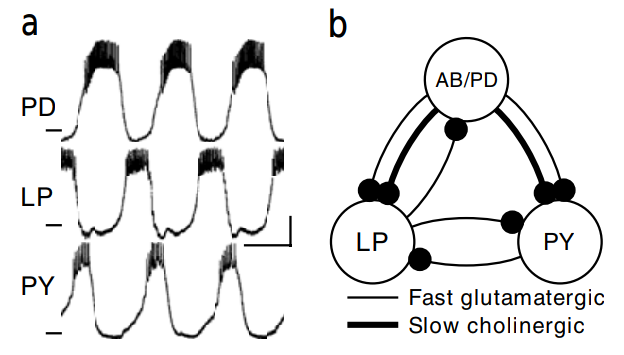
\includegraphics[width=1.0\linewidth]{gfx/prinz1}
	\caption[Pyloric network model architecture]{Biological pyloric rhythm and pyloric circuit model network. (\textsc{A}) Pyloric rhythm recorded from \textit{H. americanus} with intracellular electrodes. Scale bars, 1 s, and 10 mV; horizontal lines, -60 mV. (\textsc{B}) Schematic of a simplified version of the underlying circuit (\autoref{fig:circuitdiagram}). All synapses are inhibitory\autocite{PrinzSimilarnetworkactivity2004}.}
	\label{fig:prinz1}
\end{figure}

\FloatBarrier

\section{Modulatory Input} \label{sec:modulatoryinput}
Sharpe \textit{et al.} and Swensen \& Marder fit models of modulatory input current to experimental data. The Swensen model possesses a wider basin of activation without a sharp peak, and is based recordings from the \acs{PD} neuron. While both models fit proctolin data, \acs{RPCH} response more closely resembles the graded activation of Swensen \& Marder modulatory input.
\begin{table}[h]
	\myfloatalign
	\begin{tabularx}{\textwidth}{ccc} \toprule
		& Sharp \textit{et al.} & Swensen \& Marder \\ \midrule
		$V_{th}$ (mV) & -55 & -21 \\
		$V_\sigma$ (mV) & 5 & 8 \\
		$\tau_m$ (ms) & 6 & 6 \\
		$E$ (mV) & -10 & -22 \\
		\bottomrule
	\end{tabularx}
	\caption[Modulatory input current models]{Comparison of Sharp and Swensen modulatory input currents.}  
	\label{tab:sharpswensen}
\end{table}

\begin{figure}[h]
	\centering
	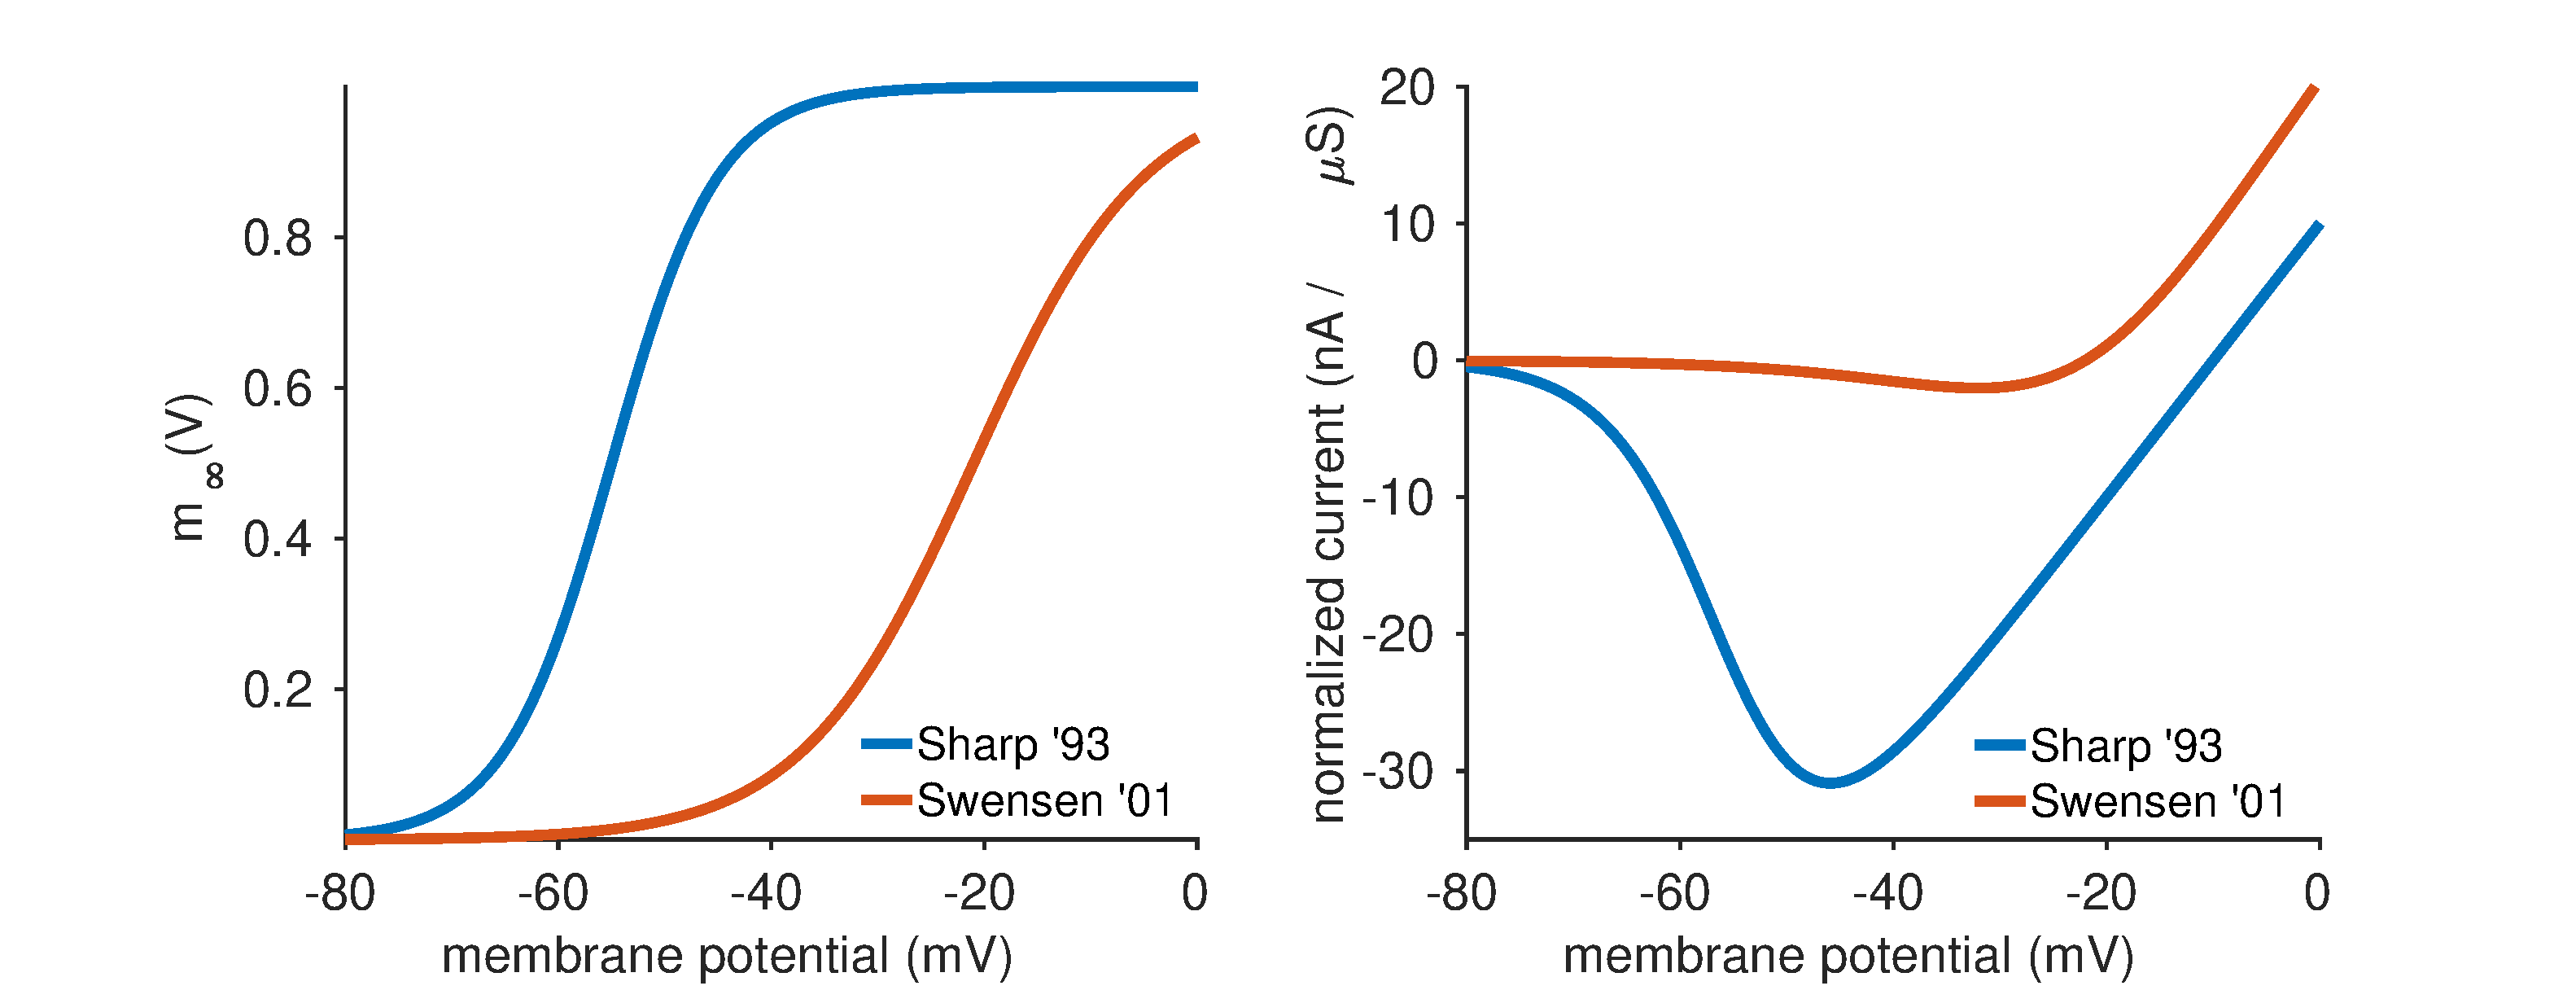
\includegraphics[width=1.0\linewidth]{gfx/SharpSwensen}
	\caption[Models of modulatory input current]{Models of modulatory input current. Sharp and Swensen modulatory input current are compared. The left-hand trace shows the activation gating variable steady-state as a function of membrane potential. The right-hand trace shows the IV curves for these model currents.}
	\label{fig:sharpswensen}
\end{figure}


\section{Model Implementation} \label{sec:modelimplementation}
In order to quickly simulate many models with varied parameters, we developed simulation software called \texttt{xolotl}. This fast single-compartment and multi-compartment simulator is written in \texttt{C++} with \texttt{MATLAB} wrappers. Designed with a focus on flexibility and speed, it can simulate single-compartment models, networks of these, and detailed multi-compartment models. This novel software has been developed by Srinivas Gorur-Shandilya and the author.

\graffito{\texttt{xolotl} is the Aztec god of lightning and death}

\texttt{xolotl} separates neurons into compartments, where each compartment and contained current is fully modular. Synapses link two compartments together. Compartments can contain any number of parameters and variables so that \texttt{xolotl} is readily adaptable to any number of simulation regimes. Since a main benefit of modeling is generating a large number of \textit{in-silico} experiments to support or generate hypotheses, \texttt{xolotl} objects can be passed through optimization protocols to develop sets of parameter values which satisfy arbitrary biological constraints. Many models can be generated which replicate biological behavior; since \acs{STG} neurons are degenerate with respect to maximal conductance density and conductance density can be assumed constant on non-homeostatic timescales, maximal conductances of intrinsic and synaptic currents serve as readily optimized parameters for single cell and network models.

Maximal conductances for intrinsic currents were bound by the interval $[0.1, 2000]~\mu \mathrm{S/mm^2}$ and synaptic conductances were bound by $[0.1,100]~\mu \mathrm{S/mm^2}$, keeping with Prinz \textit{et al.} Injected modulatory input current in dynamic clamp experiments typically lies in the range $[0,100]~\mathrm{nS}$. For this reason, maximal conductance density for \acs{IMI} was bounded by the interval $[0,1]~\mu \mathrm{S/mm^2}$ since

\begin{equation*}
	1~\mu \mathrm{S/mm^2} \times 0.0628~\mathrm{mm^2} \times \frac{1000~\mathrm{nS}}{1 \mu \mathrm{S}} = 62.8~\mathrm{nS}
\end{equation*}

Similarly, \citeauthor{SwensenModulatorsconvergentcellular2001} report the maximal steady-state current in \acs{PD} cells to be $-1.8~\mathrm{nA}$. A modeled maximal conductance of $1.0~\mu \mathrm{S/mm^2}$ would produce a current of $-2.0~\mathrm{nA}$. 

\subsection{Parameter Optimization} \label{sec:parameteroptimization}
The first step in any parameter optimization algorithm begins with the cost function $f: \mathbb{R}^n \rightarrow \mathbb{R}$. The function accepts a candidate solution in the form of a vector of real numbers and produces a real output, which represents the objective function value of the candidate solution. This process is necessary to objectively and unambiguously evaluate the fitness of a model by reducing the high-dimensional parameter set and the complicated non-analytical function which produces the resultant waveforms into a single real number. Optimization algorithms aim to discover candidate solutions which produce low costs, where a cost of zero signifies a model which fits the cost function perfectly. Since the \acs{STG} is highly degenerate in ion channel expression, maximal conductances are the targeted parameters. The solution space has been loosely characterized, producing a large number of parameter seeds to optimize.

\graffito{\texttt{procrustes} is a bandit of Greek mythology who forced his victims to fit into a bed, by stretching and amputating }

We built an optimization toolbox, \texttt{procrustes}, which optimizes any parameters passed to it based on an arbitrary cost function.  The interface serves as front-end for several parameter optimization algorithms used to develop models with desired metrics. Since application of \acs{RPCH} increases the burst frequency and maximum of the slow-wave oscillations in \acs{PD} and \acs{LP} cells, increases in these metrics over increasing modulatory input is strongly targeted. We tested \texttt{procrustes} with three parameter optimization algorithms: gradient descent, a genetic algorithm, and particle swarm optimization.

The simplest, gradient descent, is a first-order iterative algorithm in which candidate solutions take steps proportional to the gradient of the cost function at the current point. This method can readily be applied to high-dimensional spaces, though can be inefficient. Close to the minimum, gradient descent tends to ``zig-zag'' in parameter space. For a cost landscape with many local minima, many seeds with diverse parameter values must be used in order to effectively characterize possible solutions.

A genetic algorithm combines a gradient descent methods with stochastic ``mutation,'' in which solutions are combined or transformed to produce better ones. This has the advantage of more readily finding substantial local minima, but escaping from superficially fit solutions. Unfortunately, genetic algorithms are computationally expensive and suffer in problem domains with a complex cost landscape.

Particle swarm optimization relies on the generation of many candidate solutions (``particles'') which move in parameter space towards the best position of a particle in the swarm. Since the parameter space is widely sampled by the stochastically-generated particles, particle swarm optimization can efficiently handle complex cost landscapes and high-dimensional parameter spaces. Particle swarm optimization is especially effective in this case since solutions can be readily screened for non-bursting, non-triphasic activity and rejected by the swarm.

Regardless of algorithm, the greatest difficulty is almost always writing a sufficient cost function, which arrives at suitable solutions within appreciable time. Since no general technique exists for producing Lyapunov functions for ordinary differential equations; the cost function must be designed manually. A good cost function consistently produces models which satisfy the researcher's needs in efficient time. While the cost function must be ambiguous with respect to the constraints of optimization, the construction of the function and evaluation of resultant models is entirely arbitrary. \autoref{fig:procrustesexample} shows that optimization can arrive at suitable solutions in a short period of time, provided that an efficient and unambiguous cost function is implemented.

\begin{figure}[h]
	\centering
	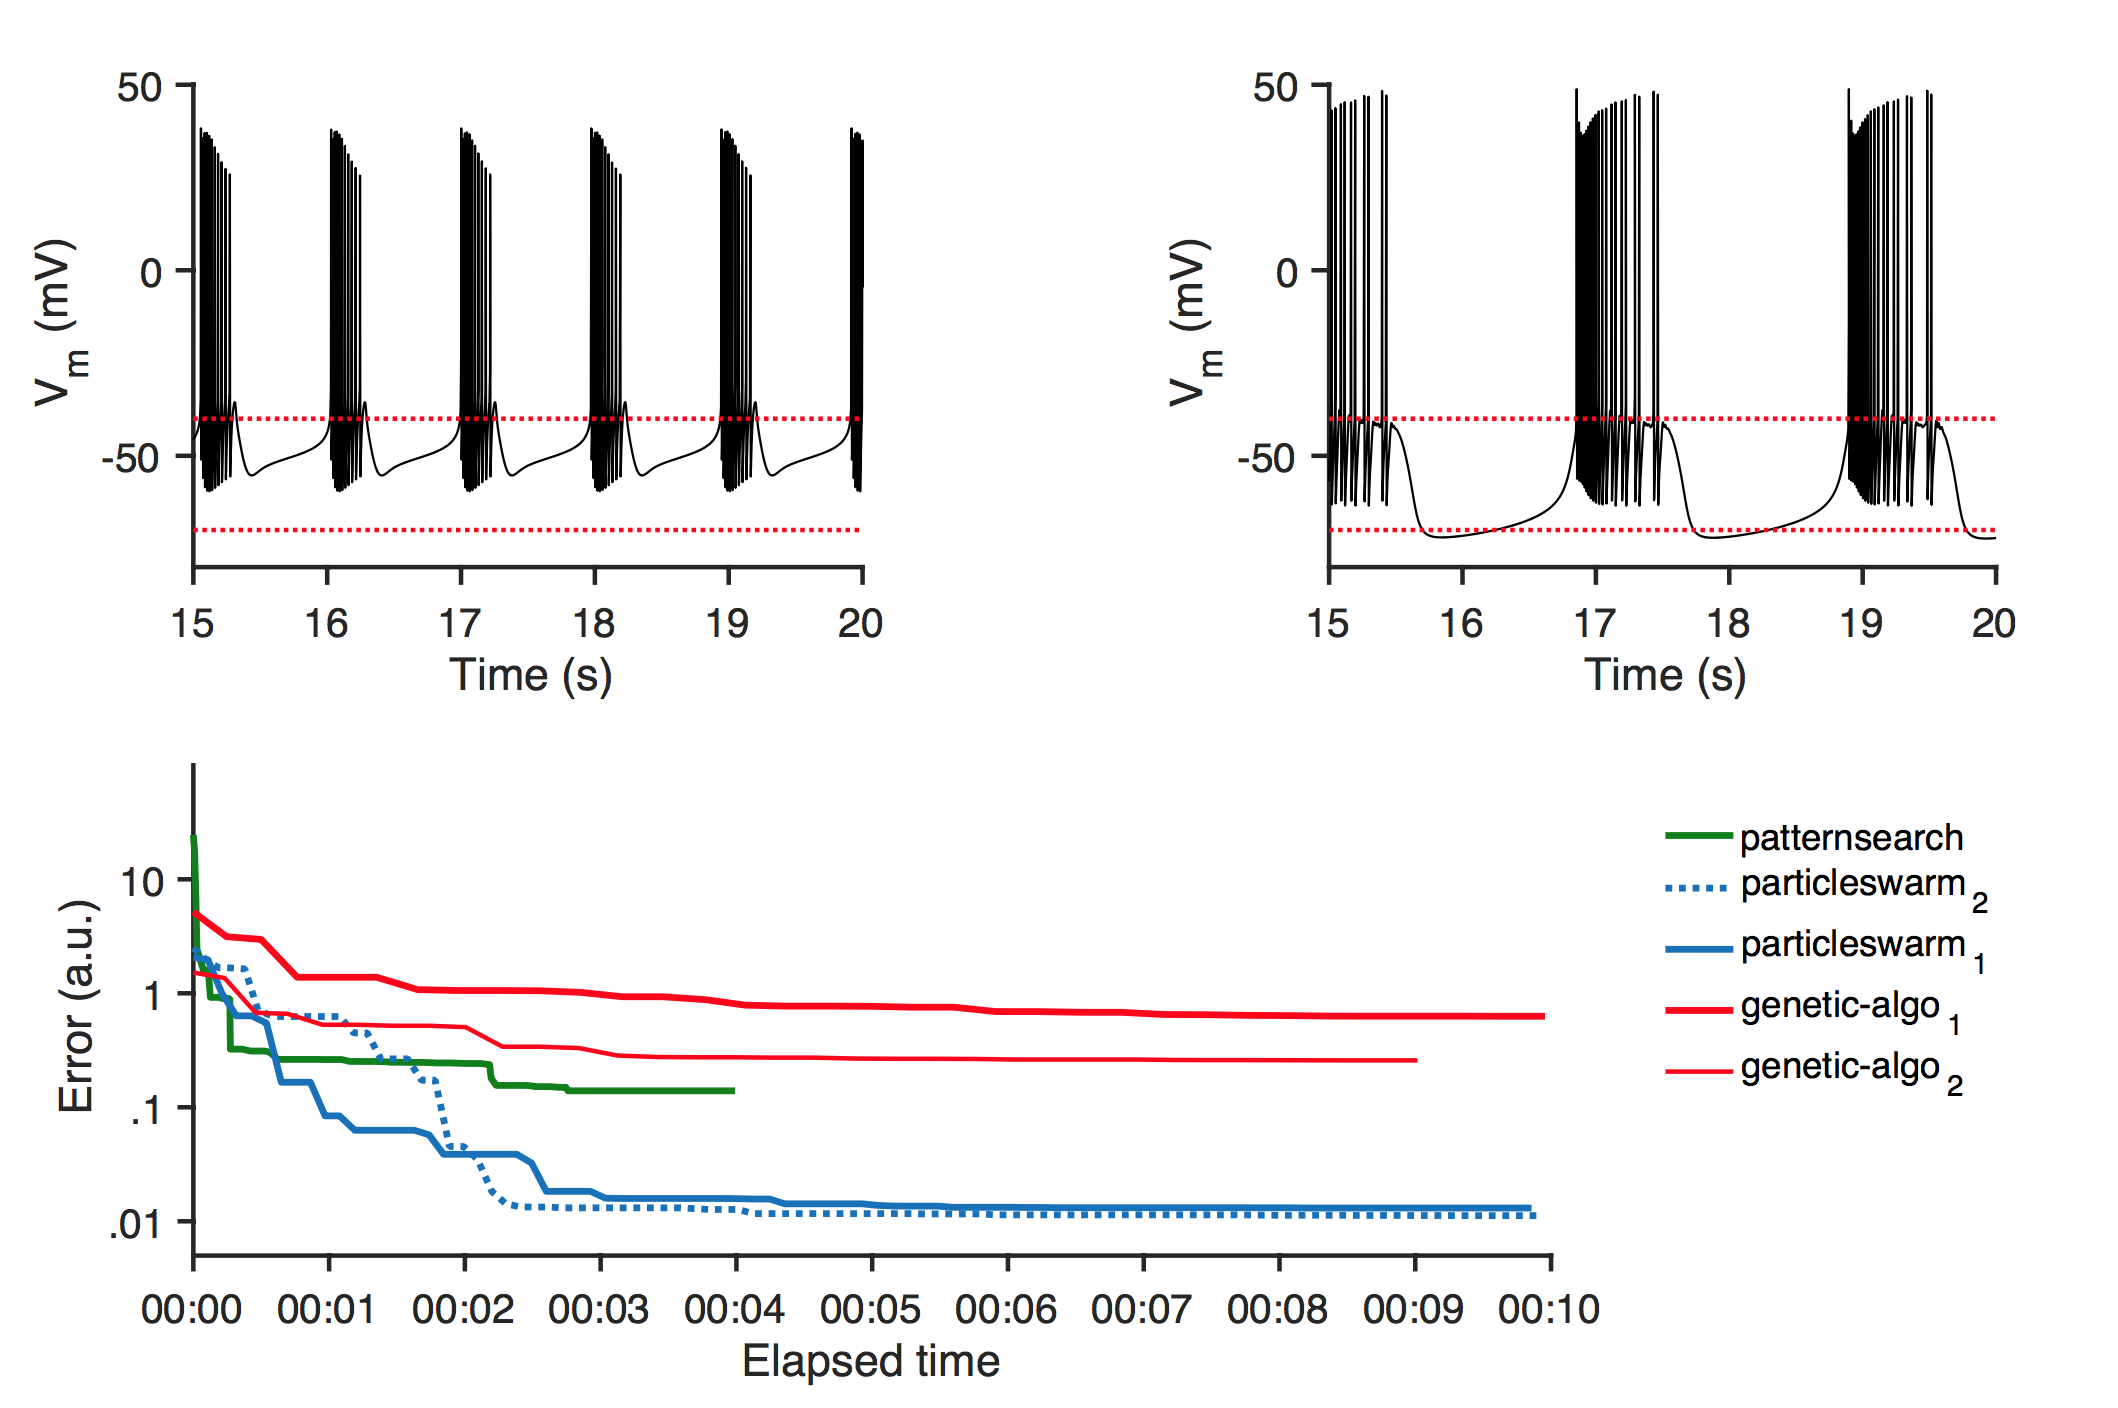
\includegraphics[width=1.0\linewidth]{gfx/ProcrustesExample}
	\caption[Parameter optimization using different algorithms]{Particle swarm optimization finds high-dimensional neuronal models with arbitrary constraints faster than other common algorithms. The top left trace displays a single-compartment seed. The top right trace displays the solution after optimization. Metrics for optimization were burst-frequency of 0.5 Hz, duty cycle of 0.3, and a slow wave bounded by $[-70, -40]$ mV where the spike troughs are above the slow wave. The bottom trace shows three optimization algorithms beginning with the same seed. Optimization terminates after 10 min or at a local minimum, as set by optimizer options. Figure by S. Gorur-Shandilya.}
	\label{fig:procrustesexample}
\end{figure}

\FloatBarrier

\subsection{Computing Metrics} \label{sec:metrics}
Simulation of a conductance-based model elicits voltage and calcium traces. The peaks of the calcium trace indicate the points of greatest spike density in the voltage traces. For a stationary signal, the burst period is the mean time between calcium peaks. The duty cycle is the ratio between burst duration and burst period. The time between the end of a burst of one cell and the beginning of a burst in another cell is the gap. Similarly, the delay is the time from a start of one burst in one cell to the beginning of a burst in another.

\begin{align}
	\mathrm{burst~period} &= mean(\mathrm{calcium~peaks}) = \frac{1}{\mathrm{burst~frequency}} \\
	\mathrm{duty~cycle} &= \frac{\mathrm{burst~duration}}{\mathrm{burst~period}}
\end{align}

\begin{figure}[h]
	\centering
	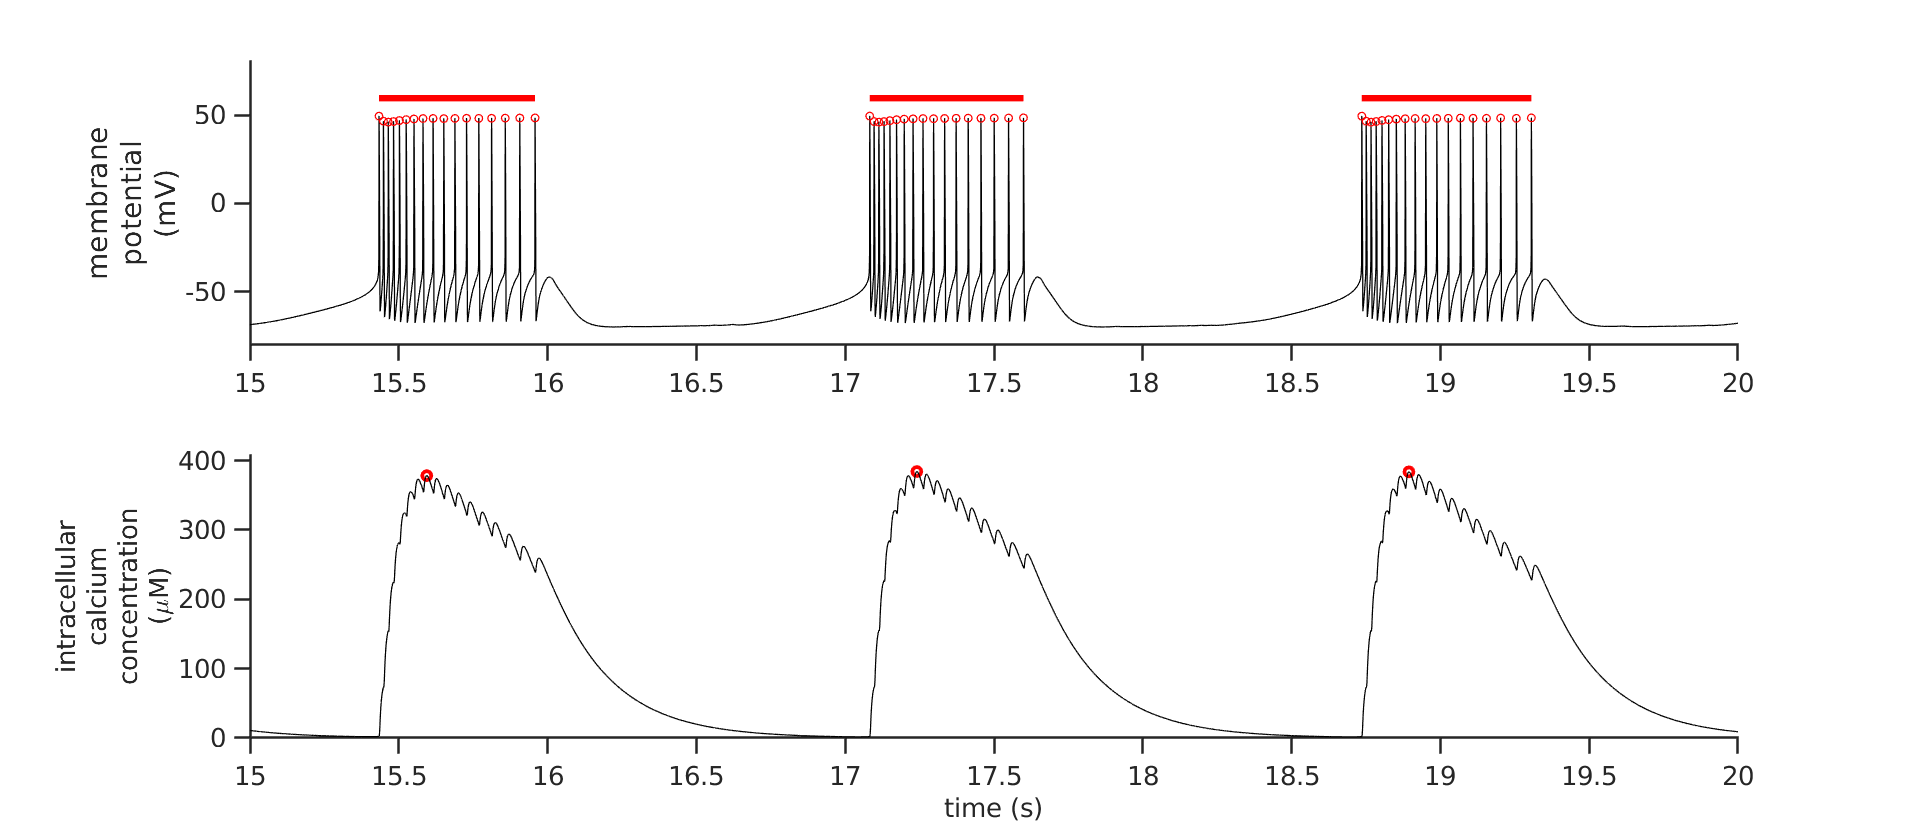
\includegraphics[width=1.0\linewidth]{gfx/BurstMetrics}
	\caption[Estimating burst metrics]{Estimating burst metrics. On the top trace, red dots show spike peak locations. The red bar indicates the burst duration. The bottom trace displays red dots at the calcium peaks.}
	\label{fig:burstmetrics}
\end{figure}

\subsection{Designing the Cost Function} \label{sec:cost}
For evaluations of three-compartment network models, the cost function computes the cost, burst frequency, duty cycle, mean spikes per burst, and the global minimum and maximum of the slow wave at several values of modulatory input into one or more cells. 

First the function evaluates whether the model elicits network activity within normal limits for real pyloric circuits. Once this has been confirmed at all steps of modulatory input current, the model targets ratios in various metrics to fine-tune solutions towards target activity.

\subsubsection{Evaluate Models for Pyloric Activity}
The first step confirms that the model is triphasic and pyloric. Burst periods, mean spikes per burst, burst durations, duty cycles, inter-burst periods, and delay between the starts of each burst were computed. If within an acceptable range, the cost was set to zero and penalized by by a normalized cost if outside the range. This range is set by experimental results. Normal pyloric networks fall within the following bounds.

\begin{table}[h]
	\myfloatalign
	\begin{tabularx}{\textwidth}{lll} \toprule
		\tableheadline{Metric} & \tableheadline{Lower} & \tableheadline{Upper} \\ \midrule
		calcium peak coefficient of variation & 0 & 0.1 \\
		burst period (s) & 0.3 & 2 \\
		spikes per burst & 4 & 30 \\
		burst duration (s) & 0.2860 & 1.4 \\
		duty cycle & 0.2050 & 0.4250 \\
		inter-burst period from \acs{AB}-\acs{PD} to \acs{LP} (s) & 0.112 & 0.33 \\
		inter-burst period from \acs{LP} to \acs{PY} (s) & -0.121 & -0.001 \\
		delay from \acs{AB}-\acs{PD} to \acs{LP} (s) & 0.6340 & 0.9720 \\
		delay from \acs{AB}-\acs{PD} to \acs{PY} (s) & 0.9250 & 1.3570 \\
		\bottomrule
	\end{tabularx}
	\caption[Pyloric network metric bounds]{Pyloric network metric bounds.}  
	\label{tab:metricsbounds}
\end{table}

For a value $v$ and target bounds $b_{low}$, $b_{high}$, the computed cost is

\begin{equation}
	\mathrm{cost} \propto 1 - \Bigg| \frac{b_{high} - b_{low}}{b_{high} + b_{low} + 2v} \Bigg|
\end{equation}

outside the bounds and zero within bounds. The first 50\% (10 s) of simulation were discarded as transient and spike times were computed by positive crossings of the zero line. If the network is bursting with an appropriate number of spikes, the model is checked for depolarization block, in which the membrane is depolarized but cannot spike. The voltage between each spike is recorded and each inter-spike interval within the burst is checked against the mean inter-spike interval for the burst to confirm that the compartment is regularly spiking during the burst. If any of these tests fail, the cost function returns a high cost and the exits the simulation.

There are several advantages to this preliminary step. First, the high cost guarantees that the failing candidate solution will not be the lowest-cost solution in the swarm, meaning that other models will not repeat the same optimization steps. Second, exiting the simulation saves time, since this solution will be discarded in any case.

As initial parameters for parameter optimization over response to modulatory input, 1,148 network models with a cost of zero in the decentralized condition were used. This dataset is available upon request.

\subsubsection{Response to Modulatory Input}
If candidate solutions pass pyloricity tests in the modulated and decentralized cases, the solution is further refined. The burst frequency, duty cycle, mean number of spikes per burst, and minimum and maximum of the slow wave are computed. A Savitzky-Golay filter with a window size of 300 ms is used to determine the maximum of the slow wave. In all other cases, the raw trace is used.

\begin{figure}[h]
	\centering
	\includegraphics[width=1.0\linewidth]{gfx/SavitzkyGolay}
	\caption[Savitzky-Golay filter visualizes slow wave]{Estimating slow wave maxima using a first-order Savitzky-Golay filter with a window of 300 ms applied to the voltage trace of a bursting neuron. A Savitzky-Golay filter is a convolutional digital filter which fits sub-sets of adjacent data to a low-degree polynomial by the least squares method. This has the effect of smoothing high-amplitude, high-frequency oscillations, without strongly distorting low-frequency signal components\autocite{SavitzkySmoothingDifferentiationData1964}.}
	\label{fig:savitzkygolay}
\end{figure}


The ratio between metrics in the modulated and decentralized case are computed. Targeting a ratio has several benefits. First, it is agnostic to initial neuron parameters. For instance, burst frequencies in healthy pyloric circuits commonly vary on the interval $[0.5, 1.5]$ Hz between preparations\autocite{MarderUnderstandingCircuitDynamics2007}. By computing a ratio, the response is normalize to the basal activity of the model, preventing over-fitting. In addition, examining two values of maximal conductance, rather than a series of linearly-spaced values significantly cuts down on computational complexity. While only two points were specified in the ratio, the constraint of pyloricity means the cost function strongly favors models with graded increase with respect to increasing modulatory input. For single-neuron simulations, this constraint does not exist.

Because the change in slow wave amplitude is a signed quantity, the slow wave maximum towards a +5 mV increase instead of a rational change.

\begin{table}
	\myfloatalign
	\begin{tabularx}{\textwidth}{lll} \toprule
		\tableheadline{Metric} & \tableheadline{Ratio} & \tableheadline{Change} \\ \midrule
		burst frequency & 1.5 & \\
		duty cycle & 1.0 & \\
		slow wave maximum & & +5 mV \\
		slow wave minimum & & -5 mV \\
		\bottomrule
	\end{tabularx}
	\caption[Pyloric network metric ratios]{Pyloric network metric target ratios and changes between the modulated and decentralized cases.}  
	\label{tab:metricsratios}
\end{table}

Graded increases, where the cost is summed for each point along the \acs{IMI} maximal conductance range, was only used for single-neuron fitting of models to dose-response data. In this regime, metric values are specified for each value of modulatory input maximal conductance. This method has the advantage of increasing the cost on models which do not exhibit graded responses to modulatory input, but is computationally expensive and may result in over-fitting.



%*****************************************
%*****************************************
%*****************************************
%*****************************************
%*****************************************
